En el presente capítulo se explica la experimentación 
realizada para la clasificación de los videos del 
\textit{dataset Hockey Fights}. La 
estructura que se detalla a continuación consiste de: 
explicación del \textit{pipeline}, preprocesamiento de 
los videos, experimentación con las diferentes configuraciones 
y comparativa de los resultados.

\section{Pipeline propuesto}

La Imagen \ref{metodologia} ilustra la metodología propuesta, 
la cual se procederá a explicar a continuación:

\begin{figure}[h!] 
    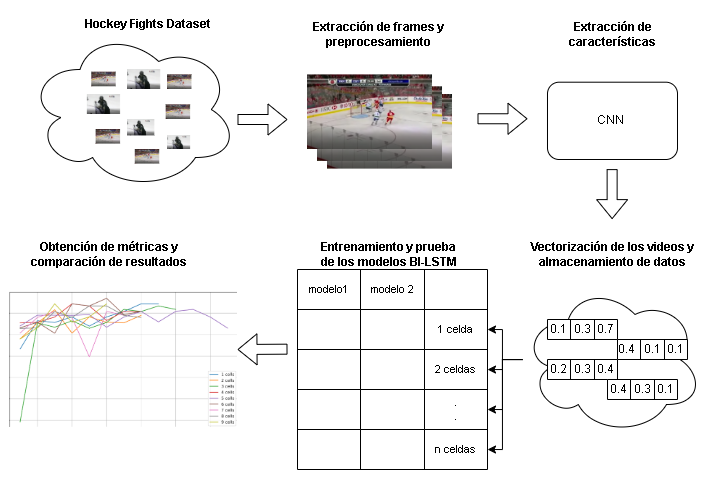
\includegraphics[width=0.7\textwidth]{images/metodologiaMaestria.png} 
    \centering 
    \caption{Metodología propuesta. Creación propia.} 
    \label{convolucion} 
\end{figure}

\subsection{Extracción de frames y preprocesamiento}



